
\documentclass[12pt]{article}

\usepackage{graphicx}
\usepackage{enumerate}
\usepackage{amsmath}
\usepackage{amsthm}
\usepackage{amsfonts}
\usepackage[left=3cm,top=2.5cm,right=2.5cm,bottom=3cm]{geometry}

%Nikola Pakages
\usepackage[printonlyused]{acronym}
\usepackage{subfigure}
\usepackage{tabularx}
\usepackage{tabulary}
\usepackage{verbatim}
\usepackage{multicol}
\usepackage{longtable}
\usepackage{lscape}
\usepackage{float}
\usepackage{xspace}
\usepackage{url}
%\usepackage{xypic}
\usepackage{listings}
\usepackage{longtable}
%\usepackage{hyperref}
\usepackage{multirow}
\usepackage{rotating}
\usepackage{amssymb}
\usepackage{gensymb}
\usepackage{amsthm}
\usepackage[ruled,vlined]{algorithm2e}
\usepackage{array}
\usepackage{cite}
\usepackage{epstopdf}
\usepackage[bookmarks=true, bookmarksnumbered=true,hidelinks]{hyperref}
%My packages
\usepackage{textcomp}
\usepackage[final]{pdfpages}
\bibliographystyle{unsrt}



% Start the document
\thispagestyle{empty}

\begin{document}

% title page
\begin{center}

\begin{figure}[th]
    \centering
		
\includegraphics[width=5cm]{pics/logo.jpg}
	\label{fig:logo}
\end{figure}

\vspace{4cm}

\LARGE \textbf {LICENTIATE THESIS PROPOSAL} \\[2cm]

\LARGE \textbf {Human Detection and Positioning in Enclosed Environments with Ultra Wideband Radar} \\[2cm]


\normalsize{Melika Hozhabri} \\
School of Innovation, Design and Engineering (IDT) \\
ITS-EASY Industrial Research School\\
Embedded Sensor Systems for Health (ESS-H)\\
M\"{a}lardalen University \\
melika.hozhabri@mdh.se \\
November 2016\\

\vspace{3cm}

\begin{minipage}{1.0\textwidth}
\begin{flushright} \small 
\textbf{Main Supervisor: Maria Lind\'{e}n} \\
\textbf{Co-supervisors: Martin Ekstr\"{o}m, Nikola Petrovic}\\
\textbf{Reviewer: Mats Bj\"{o}rkman}

\end{flushright}
\end{minipage}


\vfill


\end{center}

% table of content page
\newpage
\pagestyle{plain}
\setcounter{page}{1}
\pagenumbering{arabic}
\tableofcontents


% abstract page
\newpage

%\begin{abstract}
%Hej
%\end{abstract}

% body of the document
\newpage

\part{Thesis}
\newpage
%
%--------------------------------------------
%
\section{Introduction}
Recent advances in information technology makes it possible to create an awareness of the environment, which includes to detect and respond to the presence of a human. This might be done due to variety of reasons, such as security applications like intruder detection and collision avoidance, safety applications such as avalanche and rubble search and rescue missions, police raid operations, driving assistance, elderly care and living assistance for Alzheimer patients.
Depending on the application there are different requirements of the detection and sensing. Examples include pure determination of presence or specifying the location, tracking or identification. This theses focuses on the determination of presence and localization of human in enclosed environments. 

While machineries are becoming important in the industry, new requirements emerge, one is to allow humans to safely collaborate with robots and machines. This will increase the efficiency of sites and reduce accidents and injuries. Techniques such as infrared detectors\cite{InfraredHumanDetection}, vision based systems\cite{VisualSurveillanceBoult},\cite{Visualhumandetection}, vibration and seismic waves\cite{VibrationTracking}, acoustics\cite{AcousticsHumanDetection} and radar sensors\cite{YarovoyUWBHumanDetection} are used as a solution to human detection problem.

Some systems are built based on the fusion of these sensors to take advantage of each sensor strength to increased confidence of detection and decrease false alarms.
In\cite{RadarVisionfusion} Milch and Behrens used radar-vision fusion for detecting pedestrians on-board a moving vehicle. Radar sensor is used to generate a target list or hypotheses for presence of pedestrians. In the next step vision system is used to prove the hypotheses, if the target is a pedestrian. 

Human detection using radar has advantages such as the ability to function in all lightning conditions whereas visual, infrared and laser sensors are prone to fog, smoke, dirt, environment’s lighting conditions or temperature changes. In addition visual, infrared, and seismic sensors need to be placed in close proximity to the target whereas radar senors depend on frequency of the operation can function up to several hundred meters.

The human detection with radar has two main tasks: first the target shall be detected then it shall be decided if the detected target is a human or not. It has been different approaches in how to discriminate a human target from the other detected targets. In many of sensor fusion solutions that radar is a part of, other types of sensors are responsible for the determination whether the target is a human or not because the radar is considered to be incapable of making such decisions. The problem with this approach is that the benefits of radar sensors are not fully taken advantage of. This thesis is aiming at using the radar sensor as a stand alone solution for the whole human detection problem. This means that both detection and discrimination of the human from other targets is performed by the radar sensor. 
  
\section{Background}

Radar (RAdio Detection And Ranging) uses electromagnetic waves from a transmitter and when it interacts with an object a part of it reflects, absorbs and scatters depend on the frequency of wave, the shape and material of the object and the orientation of the incident wave. The reflected wave is different from the transmitted wave in frequency, time delay and amplitude. The frequency shift is the result of the Doppler effect due to the relative speed of the radar and the target. The time delay is due to the time it takes for the waves to travel from the radar transmitter to the object and back again. Attenuation of the signal is a result of path loss over the traveling distance by the wave. The received signal power by the radar is defined by the radar equation \ref{eq:radareq}.
\begin{equation}\label{eq:radareq}
	P_{r}= \frac{P_{t} G_{t}}{4\pi R^{2}}\times\frac{\sigma}{4\pi R^{2}}\times A_{e}
\end{equation}

The equation is written based on the product of three factors: The first fraction in equation \ref{eq:radareq} represents the power density at distance R from a radar that transmits with the power of $P_{t}$ from an antenna with the gain of $G_{t}$. The second fraction contains $\sigma$ which is radar cross section of the target and is the measure of the energy reflected from the target back to the radar. The last term in equation \ref{eq:radareq} is  $A_{e}$ which is the receiving antenna effective area\cite{skolnik2008radar}. 

%The difference between traditional radio technolgy and ultra wide band
The majority of traditional radar system are based on a narrow band signal modulated on a sinusoidal carrier wave. The amount of information that this radio systems can carry is limited due to limited bandwidth. To increase the information amount wide band and Ultra Wide Band(UWB) signals shall be chosen. This is possible due to usage of the narrower pulse in order of nano seconds, which will increase the accuracy of target range and the ability to detect smaller targets and more detailed information about them. In addition it will reduce the passive interference from for example rain and other particles due to relative reduction of scattering cross section of interference to the target\cite{taylor2000ultra}.

%Narrow band radar systems use sinusoidal signals which tend to keep their shape during signal conversions such as addition and differentiation. Because ultra wideband signals has different waveform the shape can change during signal conversion.(This part shall be added later in the licentiate)

%why UWB is better that other radar systems
UWB technology is a promising technology due to high spatial resolution and obstacle penetration capabilities. Over the past two decades the advancements in electronics made it possible to develop UWB radar system with advantages to other conventional technologies\cite{UWBHussain}.

Based on Federal Communications Commission (FCC) definition a signal can be defined as UWB signal if the fractional band with is greater than 0.2 where fractional bandwidth is defined in equation \ref{FracBW}.
\begin{equation}\label{FracBW}
	B_{f} = 2\frac{f_{H}-f_{L}}{f_{H}+f_{L}}
\end{equation}
%Some active localization system require the person carry a radio-frequency tag
%The disadvantage is that the data is not possible to be visualized for a human eye contra vision system
%detection relies on the back-propagation of the signal from the body
Different types of UWB radar are developed and based on the excitation wave-form they are divided to different categories. Three of the most prominent categories are Frequency Modulated Continuous Wave (FMCW), pulse and M-sequence. In this research we have access to a commercially available M-sequence UWB radar which is developed in Radarbolaget. Radarbolaget is positioned in G\"{a}vle, Sweden developing radar
systems primarily for real time, through wall monitoring of heating furnaces \footnote{http://www.radarbolaget.com}.To be able to understand the system constraint a comparison study between UWB M-sequence and pulse is done in paper A. The pulse radar belonged to Time Domain\textsuperscript{TM}, one of the leading companies in developing UWB radar and communication systems \footnote{http://www.timedomain.com}. Sachs et. al. compared pulse and M-sequence for UWB technology in\cite{sachs2003stimulation}. Based on technical specifications of each system it is reasoned that the pulse based
UWB systems are desirable in applications with simple data interpretation and low power consumption versus the M-sequence based approach needs more complicated data processing but provides highly stable data.


%As humans are made of 70\% water a good part of this waves reflect back to the receiver. 
%The frequency of th radar also can determine the size of the detectable object. The lower the wave length the smaller the detectable object. traditional radar devices send a wave with a small frequency band and in the receiver the reflected signal can be processed and filtered by that specific frequency.
%the goal of research questions or 
%research challenges are sensing noise, environment variation\cite{Teixeira2010}.
%different types of clothing, hats, backpacks, purses, and\cite{Dogaru2007} \cite{Yamada2005}
.
%
% --------------------------------------------
%

\section{Related Work} 
In this research first the system characteristics have been thoroughly investigated and measured. Two of the main focused characteristic were the ability of the sensor to differentiate a human body from other materials and the effect of the environment noise on the signal detection. Second, suitable signal processing algorithms has been developed and implemented which can extract features specific to human such as breathing to discriminate a living human from other targets detected by the radar . 
 
\subsection{Human Radar Cross Section }
To be able to quantify target echo in terms of  the target characteristic, a term called Radar Cross Section(RCS) is defined. The RCS is the projected area of a metal sphere that would return the same echo signal as the target. As mentioned earlier echo of the object depends on the size, material and direction of the incident wave. Radar cross section of the simple bodies can be computed by solving the wave equation, but for more complex objects the exact solution is not computationally feasible. Alternative approaches like method of moments or approximate methods are used. The real world applications can not rely entirely on computations and approximation so the echo measurements shall be done to get a better grasp of reality. This is done by placing the real target or a target model at radar vicinity in free space or an anechoic chamber and measure the reflections\cite{skolnik2008radar}. Dogaru et.al.\cite{Dogaru2007} modeled the radar signature of the human body. They used the human body computer model in various postures in the frequency range of 0.5 GHz to 9 GHz and all azimuth aspect angles. It is observed that for most frequencies, the RCS of the body is in a range between –10 and 0 dBsm, where dBsm is a notation for RCS of a target in decibels; 1 m2 corresponds to 0 dBsm. It also shown that the posture and amount of fat on the body can affect the RCS, but the average remains the same for different postures. One reason for this is because the main contribution of the radar reflection is typically coming from the trunk.
In \cite{Yamada2005}, N. Yamada et al measured the RCS for a human in a band at 76 GHz. While the RCS is changing with orientation, the average intensity was found to be –8.1 dBsm, and as expected, the front and back produced the largest reflection. It is also shown that the type of clothing being worn can then affect the radar reflection.
Paper B contains measurements of human and human model backscatter and it is planned to include same type of measurements in paper C.

\subsection{Environment Noise}
Clutter is all unwanted radar return signals. A part of this research is focusing on highly cluttered environment like mines so it is needed to understand the effect of clutter on signal detection. Clutter in a mine is formed by walls, floors, machineries i.e. by anything but the human in the scenario. Sources of clutter can be out-of-band interference which contains frequencies other than dedicated bandwidth for the system or in-band interference and thermal noise. Ou-of-band interference can be detected and removed by traditional techniques such as Fourier transform and bandpass filter. In-band interference is harder to identify and to remove. Clutter can affect the probability of detection and accuracy. To understand and quantify clutter the statistical properties of the clutter are often used. A statistical radar clutter model for modern high resolution radars is presented in \cite{clutterModel}. Densities such as Weibull or log-normal[\ref{eq:LogNormal}] distributions are shown to provide reasonable fits for measured clutter densities.
\begin{equation}
f_X(x;\mu,\sigma) = \frac{1}{ x\sigma \sqrt{2 \pi}}\, e^{-\frac{(\ln x - \mu)^2}{2\sigma^2}},\ \ x>0
\label{eq:LogNormal}
\end{equation}

\subsection{Signal Processing}
%To ease the prototyping and experimentation process the application softwares has a specific architecture. Data acquisition and GUI software are developed in C\# and the signal processing algorithms are developed in Matlab\textsuperscript{TM} then an API connects Matlab\textsuperscript{TM} code to the GUI so after building DLLs it is possible to run the developed algorithms with real system. Matlab\textsuperscript{TM} is a prototyping platform with thousand of ready libraries and function which makes development and testing of algorithms faster. 

In general it is possible to divide the human detection with UWB radar into two categories: Behind obstacles and free space detection. Microwave in lower frequency range can penetrate most building materials whereas the higher frequency waves are capable of detecting small movements such as  breathing or heart beat. Due to the wide band width of UWB radars these two features were combined and UWB radar is used in applications such as police raid operations or rescue operations for searching under rubble after earthquakes. UWB radar is a better candidate than search dogs because search dogs can not differentiate between dead or alive people and can waste valuable time of the rescue team. In police raid operations the knowledge of criminals positions and number inside a building can bring valuable information to the operation\cite{trappedpeople}, \cite{ThroughWallHuman}. 
%We could easily confirm this by placing a person in front of the radar system breathing normally. The result was filtered with a band-pass filter and the breathing could be detected. Unfortunately it was not possible to use the same algorithm for moving human. The reason could be that the more dominant movement during walking such as moving arms or legs are masking the chest small movement.   

In\cite{SChangUWBHumanDetection} S.Chang et.al used a database to record features in radar return such as cross section size and velocity of the target and used this database to to classify human targets. In \cite{MicroDopplerGaitTahmoush} D. Tahmoush and J. Silvious extract the radar micro doppler signals generated by human motion and extract of gait features from it.

To be able to extract the human target signal, raw radar data passes several signal-processing steps. This signal usually is affected by noise, clutter and attenuation. In UWB radar based systems a big part of of signal processing is done in the time domain rather than frequency domain. In\cite{SignalProcessingSteps} all required phases of the radar signal processing is segmented and described.

\subsubsection{Background Subtraction}
Background subtraction techniques are used to reduce stationary clutter such as antenna coupling and environment static clutter. 
Background subtraction techniques could have different complexity based on application, speed accuracy and memory requirement. M. Piccardi in \cite{BackgroundsubtractionVision} provides a review of background removal methods in computer vision application but the same techniques can be applied in radar context. In this thesis two methods were investigated for background subtraction. The first one is concerning detection of static objects, a measurement of the background before the object is placed in radar vicinity is done. The average of the radar frame in every point is removed from the raw radar data after the static object is placed in the radar vicinity. This method has it's drawbacks because it does not consider the shadowing phenomena The existence of the static object will change the reflection from all the other static objects in the scene :
Background and static object - background $\neq$ static object

The second one deals with detecting moving object. Exponential averaging method is used due to its low complexity and good performance\cite{DetectionMsequenceZetik}. In this method, the clutter estimated from the previous radar sweeps and updates is removed from the actual radar measurement at the moment.
\begin{equation}
S_{t} =\alpha .Y_{t} + (1-\alpha).S_{t-1}
%\label{eq:ExpoAver}
\end{equation}
Where $\alpha$ is a coefficient between 0 and 1, $Y_{t}$ is the signal and $S_{t}$ is the exponential average at time t. $S_{1}$ can be set to the first signal value. 

\subsubsection{Detection}
Detection step is about making a decision between two hypothesis: if the signal scattered from target is absent or present in radar data. In most cases the solution is using statistic theory to test the hypothesis against a threshold. The result of this decision is a binary data where 1 means that the target is probably present in the radar scan and 0 indicates the lack of target. Detection algorithms for UWB radar are discussed in \cite{taylor2000ultra}. Common solution to detection problems are (N,K)-detector\cite{NKDetector}, the interperiod-correlation processing (IPCP) detector\cite{IPCPdetector}and the constant
false alarm rate(CFAR) detector\cite{NezirovicDetectionTrappedVictims},\cite{CFARDetectionClutter}.

\subsubsection{Localization}
Time of Arrival(TOA) of the detected target is available in every radar scan. This is the time that it takes for the wave to travel from the transmitter to the target and scattered back again to the receiver. The one dimentional location is calculated by equation \ref{eq:TOA}. 
\begin{equation}
\label{eq:TOA}
	\textnormal{Distance to the target} = \frac{TOA * C}{2}
\end{equation}
where C is the speed of light.
For 3D position estimation in a coordinate system at least 4 anchor nodes are needed otherwise the ambiguity will occur. Position estimation methods can be divided into two categories: iterative and non-iterative methods\cite{UWBLocalization}. Direct Method(DM)\cite{LocalizationDM}, Least Square(LS)\cite{leastSquaresLocalization} and Spherical Interpolation(SI)\cite{SphericalInterpolation} are some of the non-iterative approaches to solve position estimation problems. Taylor Series method is an example of iterative approach for localization\cite{LocalizationTaylorSeries}.

\subsubsection{Tracking}
Tracking algorithms are often used to increase the precision of the localization results for moving targets. Most of the tracking algorithms can make an educated guess about target's next position and reduce the measurement's uncertainty and smoothen the target trajectory. Kalman filter, linear least square and particle filter are widely used in this application\cite{KalmanTracking},\cite{ParticleFilter}.

%localization and tracking with radar sensors can be device free or with active or passive tags 


%
% --------------------------------------------
%
\chapter{Contribution}
\section{Summary of The Research Work throughout Paper A-C}
\section{Contribution of Included Papers}
\label{papers}
\begin{itemize}
	\item \textbf{Paper A} \textit{Experimental Comparison Study of UWB Technologies for Static Human Detection}\\*
	Melika Hozhabri, Magnus Otterskog, Nikola Petrovic and Martin Ekstr\"{o}m\\*
	IEEE International Conference on Ubiquitous Wireless Broadband (ICUWB 2016), Nanjing, China.
	
	Abstract and Contribution:This paper compares two dominant Ultra Wide Band(UWB) radar technologies Impulse and M-sequence for static human being detection in free space. The hardware and software platform for each system is described separately. These two radar platform performances are tested in real conditions and the results show that M-sequence UWB radar is better suited for detecting the static human target in larger distances.
	
	Author's contribution:
	I have been the main author of this paper and a major part of the idea was mine. I have planned and performed the measurements with help of Radarbolaget that provided the hardware. I wrote most of the paper and analyzed the results.
	
	\item \textbf{Paper B} \textit{Study of Environment Effect on Detection of
		Walking Human by M-Sequence UWB Radar }\\*
		Melika Hozhabri, Per-Olov Risman and Nikola Petrovic
		2016 IEEE Conference on Antenna Measurements \& Applications (CAMA)
		
	Abstract and Contribution: This paper presents an experimental comparison study of human movement and presence detection in different environments using ultra-wide-band (UWB) M-Sequence radar. The benchmarking measurements are made in an anechoic chamber and repeated in an open office environment. The wave forms of the background noise and scattered amplitudes of a human body are measured and compared. A set of detection algorithms and filters which are developed to track the human movement and presence is presented and the tracking results in these two environments are compared to each other.

	Author's contribution:
	I have been the main author of this paper. I have planned and performed the measurements with help of Delta that provided the semi-anechoic chamber. I wrote most of the paper and partly analyzed the results. I partly developed the signal processing algorithms and filters.  
	\item\textbf{Paper C} \textit{Comparison of UWB Radar Backscattering by the
    Human Torso and a Phantom}\\*
		Melika Hozhabri, Per-Olov Risman and Nikola Petrovic
		2018 IEEE Conference on Antenna Measurements \& Applications (CAMA)
		
	Abstract and Contribution: An Ultra Wide Band (UWB) radar is used to measure the backscattering of a human and a human phantom. The choice of material and shape for the human phantom is discussed. The dielectric properties of the material (wet sand) used in the experiment are measured by a retromodeling technique and also calculated by mixture formulas. The appropriate frequency choice for the application is discussed.
	
	Author's contribution:
	I have been the main author of this paper. I have planned and performed the measurements with help of Radarbolaget in G{\"a}vle University that provided the radar hardware and . I wrote most of the paper and partly analyzed the results.\todo{change this abit, write about what PO did?}
	
\end{itemize}
To be able to understand the system constraint a comparison study between UWB M-sequence and pulse is done in paper A. The pulse radar belonged to Time Domain\textsuperscript{TM}, one of the leading companies in developing UWB radar and communication systems \footnote{http://www.timedomain.com}. Sachs et. al. compared pulse and M-sequence for UWB technology in \cite{sachs2003stimulation}. Based on technical specifications of each system it is reasoned that the pulse based UWB systems are desirable in applications with simple data interpretation and low power consumption versus the M-sequence based approach needs more complicated data processing but provides highly stable data.
%
% --------------------------------------------
%
\section{Research Method}

To be able to define a research goal, this work started by a systematic literature review in order to know the state of the art and to recognize the requirements and challenges. In addition, industrial partners in robotics and mining industry to Addiva AB have been consulted in the matter, in order to achieve a better understanding of the real world challenges that each particular industry is facing with.
%\footnote{This research is partly financed by Vinnova Diarienummer 2014-00484} 
One prerequisite of the work was to use an already existing hardware system for the UWB radar. The second part of the literature review was mostly about understanding the existing hardware and its advantages and limitations. The research method used in this thesis was an induction method. It means that the experimental result leads to forming a theory. Series of experiments is performed and collected data was analyzed which resulted in scientific papers and better understanding of the system. This has been an iterative process as each result led to more knowledge which in turn resulted in new literature studies and set of experiments.
    
% The research goal is solving concrete problem so identifying the research goal was the first step.  

%
% --------------------------------------------
%
\section{Research Goal}
\label{ResearchGoal}
The purpose of this research is to develop a system being able to protect humans around dangerous machinery in environments like mines that conditions such as lack of light, dirt and fog cause other technologies decrease in functionality. This feature is needed in mining industry where safety requirements around automatic machineries are getting more stringent to help protecting human lives. 
%Of course the same technique can be used in other applications such as pedestrian collision protection in self driving cars.
The research goal for this thesis is:

\textit{"To design, assemble and evaluate a wireless system to be able to detect and localize humans in enclosed environments."}

This general goal can be broken down by following research questions.
\begin{enumerate}
\item [RQ1] {What are the advantages and drawbacks of the UWB radar in comparison to other sensors used in this particular application?}\\ 
\item[RQ2] {What are the characteristics of the background noise? How and how much will this noise effect the signal detection?}\\ 
\item[RQ3] {What are the algorithms to be used for detection of human with the chosen sensor?}\\
\item[RQ4] {What is the chosen sensor performance in terms of false alarms and missed detection?}\\ 
\end{enumerate}

%
% --------------------------------------------
%
%\section{Ethics}
The ethical discussion in this research can be divided in two 
In passive positioning the identity of the person is not revealed
If the person carries a tag 
Realtime positioning and localization  
The issue is worsen as with this particular radar technique the act of surveillance can be performed without consent as the electromagnetic waves can penetrate the obstacles and walls.
the data can be used to predict user movement
Dobson and Fisher used the term “Geoslavery”\cite{Dobson2003} and say “practice in which
 one entity, the master, coercively or surreptitiously monitors and exerts control over the
 physical location of another individual, the slave.” and “the challenge is to develop safeguards that simultaneously permit
 legitimate uses while preventing mis-uses
 it is convinient and safe but it can be used by terrorists and sex offenders
 Alzheimer’s patients, parents and firefighters
 
 who owns the information 
 how the information is saved
 is the information accurate enough to take decisions based on it
 who is accountable for the decision
 who have access to the information
 \subsection{Ethical Discussion}
 \subsubsection{privacy}

 \subsubsection{accuracy}
 
%
%



\section{Summary and Conclusion}

As this research is performed in collaboration with industry, it faces a real world application where the requirements are well defined and rigid, where a false alarm can be costly in robotic or a mining applications, a missed target means injuries and loss of lives. 
A successful target detection is a combination of two parts, first the chosen system hardware/technology should able to detect the target under defined requirements for the environment it is intended to be used in. The second part is dealing with the filtering and processing on the acquired data and how efficient they. Because of this the research focus has been to investigate what the system is capable of, it's constraints and processing of the obtained signals. This has so far resulted in two peer-reviewed publications. The areas that have been looked into are radar signal processing in time domain, statistical signal processing and detection theory. There are several challenges for reaching the research goal(see \ref{ResearchGoal}). Based of the last measurements in the office environment and published in paper B the probability of false alarm is around 50 percent. This is not a satisfactory result and needs further investigation. In addition discrimination of a human from other object is not an easy task. Applying the breathing filter to a walking human could not deliver satisfactory results due to the bigger movement of other body parts masking the chest movement. 

\section{Future work}
Some planned future work before the PhD thesis are listed below:
\begin{itemize}
	\item During this research some of the system characteristics such as precision and effect of environment noise in signal detection were measured and defined whereas some other characteristics such as maximum range needs to be measured and defined.
	\item   Further investigation is needed to figure out how much of the high percentage of the false alarm depends on the signal processing algorithms and how much is system/hardware dependent.
	\item For discrimination between human and other objects some other types of approaches such as micro doppler processing needs to be tested.
\end{itemize}

\newpage
\section{Preliminary Outline of the Thesis}
\begin{enumerate}
	\item Title
	\item Abstract
	\item Table of Contents
	\item Part I: Thesis
	\begin{itemize}
		\item Introduction
		\begin{enumerate}
			\item Motivation
			\item Research Questions
			\item Background
			\item Related Work
		\end{enumerate}
		\item Research Methodology
		\begin{enumerate}
			\item Research Process
			\item Research Methods
			\item Research Approach in the Future Work
		\end{enumerate}
		\item Thesis Contribution
		\begin{enumerate}
			\item Summarizing Discussion
			\item Conclusion
			\item Future Work
		\end{enumerate}

		\item References/Bibliography for Part I
	\end{itemize}
	\item Part II: Included Papers
	\begin{itemize}
		\item Paper A
		\item Paper B
		\item Paper C
	\end{itemize}
\end{enumerate}

%
% --------------------------------------------
\newpage
\part{Graduate Education}
% --------------------------------------------
\newpage
%
\section{Courses}
\label{Courses}
Courses that are taken for the graduate education are listed below. Each student is required to pass 45 points for licentiate thesis.
\begin{center}
	\begin{tabular}{| l | l | l |}
		\hline
		\textbf{Course Name} & \textbf{Credits} & \textbf{Status} \\ \hline
		Case Based Reasoning & 15 & Completed \\ \hline
		Estimation Theory & 10.0 & Completed \\ \hline
		Antenna Theory, PhD Course I & 8.0 & Completed \\ \hline
		Professional Ethics & 7.5 & TBD \\ \hline
		Scientific Writing with LaTeX & 7.5 & TBD \\
		\hline
		Reseach methodology & 7.5 & Completed \\
		\hline
		Research Planning & 3.0 & Completed \\ \hline
		Training School on UWB Antennas, Technologies and Applications & 1.5 & Completed \\ \hline
		\multicolumn{1}{r}{\textbf{Sum =}}&\multicolumn{2}{l}{\textbf{60}} \\
	\end{tabular}
\end{center}

\section{Conferances and Workshops}
I attended following conferences during my graduate education: 
\label{Conferances}
\begin{itemize}
	\item 2014 IEEE International Conference on Ultra-WideBand (ICUWB)
	
	I attended this conference in Paris and I got acquainted with the experts in the field and get a holistic view of state of the art research in the field.
	\item Training School on UWB Antennas, Technologies and Applications - Karlsruhe, Germany, April 20-24
	
	This training school was arranged by European school of antennas and COST action TU1208 for ground penetrating radar(GPR). The training was giving an insight to UWB antennas and system by the prominent researchers in the field.  
	\item 2016 IEEE International Conference on Ubiquitous Wireless Broadband (ICUWB)
	I attended this conference to present paper A.
\end{itemize}



\subsection{Third cycle outcome}

\subsubsection{Knowledge and understanding / Research Area}
 \textbf{1.1a Knowledge and understanding of the research area}

I have taken graduate courses (see \ref{Courses}), attended one licentiate and one PhD defense and presentation. I attended a training school and conferences (see \ref{Conferances}).

 \textbf{1.1b Specialist knowledge in a defined part of the research area}
 
 I have published peer reviewed- scientific papers and participated in international workshops and conferences.
 
 \textbf{1.1c Deep knowledge of research methods in general, and of research methods in the specific research area}

I have taken research methods and research planning courses.

\subsubsection{Competence and Skills}
\textbf{2.1a Critically and independently identify and formulate research questions}

I have written and published scientific articles and papers as first author and main contributor (see \ref{papers}).

\textbf{2.1b Contribute to the development of knowledge}
I have performed studies and experiments and published the results in scientific articles and papers (see \ref{papers}).

\textbf{2.2 Orally and in writing present and discuss research results with the national and international scientific community, and the society in general}
I have written and published scientific articles and attended with own contributions at international conference(see \ref{papers}).

\textbf{2.3 Independently conduct research and development}
I have been the main responsible for this research and published peer reviewed scientific articles. 

\subsubsection{Judgement and Approach}

\textbf{3.1 Demonstrate ability to make ethical assessments in own research}

I have planned my own research. I took  research ethics, research methods and research planning courses.

\textbf{3.2 Demonstrate understanding of science's role and use in society, including its possibilities and limitations, and responsibility of its use}
If this technique is going to be used in application which are protecting humans from machineries it's limitations shall be fully explored because every decisions based on the sensor data can be either costly in case of false alarm or injuries and loss of lives in case of missed target.

\textbf{3.3 Identify one's need of further knowledge and take responsibility for one's learning} 

???



\subsection{Time plan}
This is the time plan up to the licentiate seminar.
\begin{itemize}
	\item Licentiate proposal - 24 November, 2016.
	\item Professional Ethics course to be finished - Fall 2016.
	\item Scientific Writing Using LaTeX course to be finished - Fall 2016.
	\item Paper C - fall 2016. Journal paper.
	\item Application for licentiate seminar - 22 March, 2017.
	\item Licentiate thesis, first draft - Jun, 2017.
	\item Licentiate thesis, camera ready - August, 2017.
	\item Licentiate seminar - September, 2017.
\end{itemize}


\subsection{Thesis opponent and committee}
%
% --------------------------------------------


\newpage

\bibliographystyle{abbrv}
\bibliography{Licenciate}
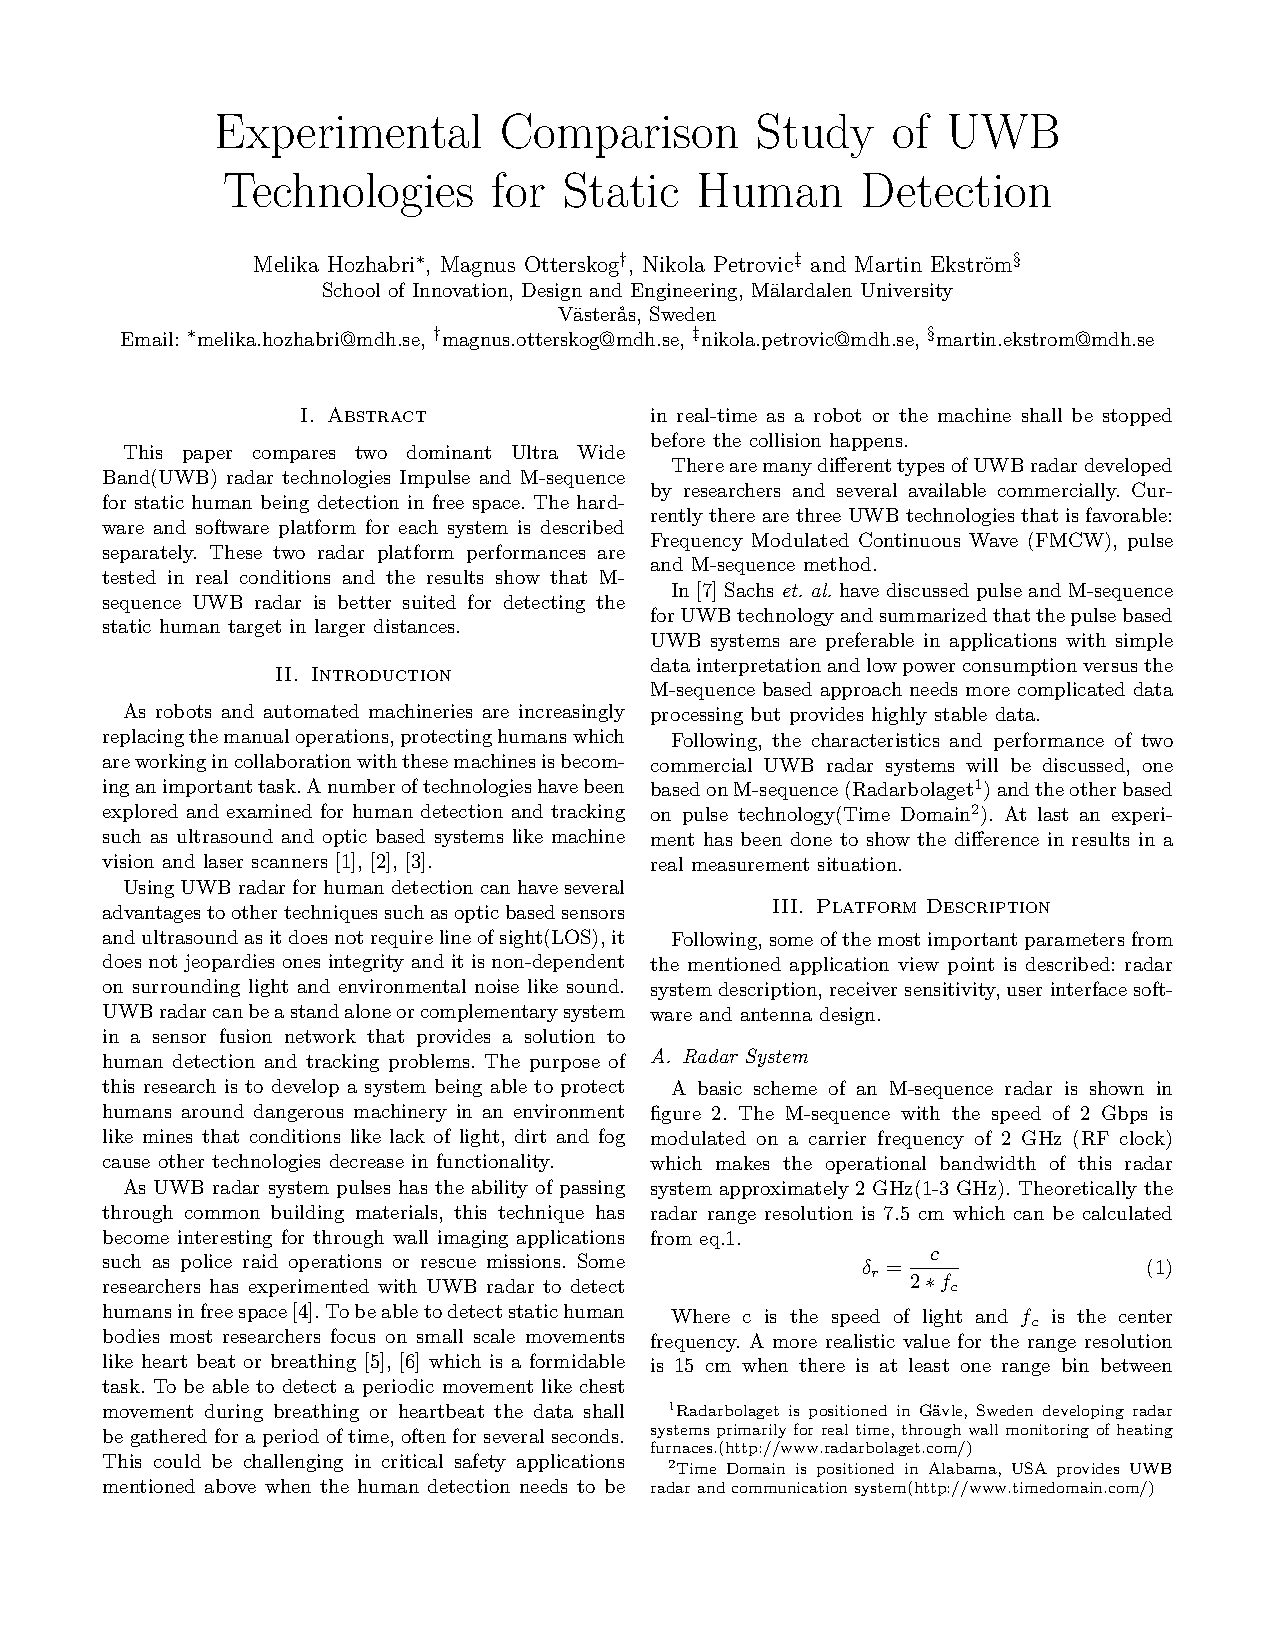
\includepdf[pages=-]{PID4265735.pdf}
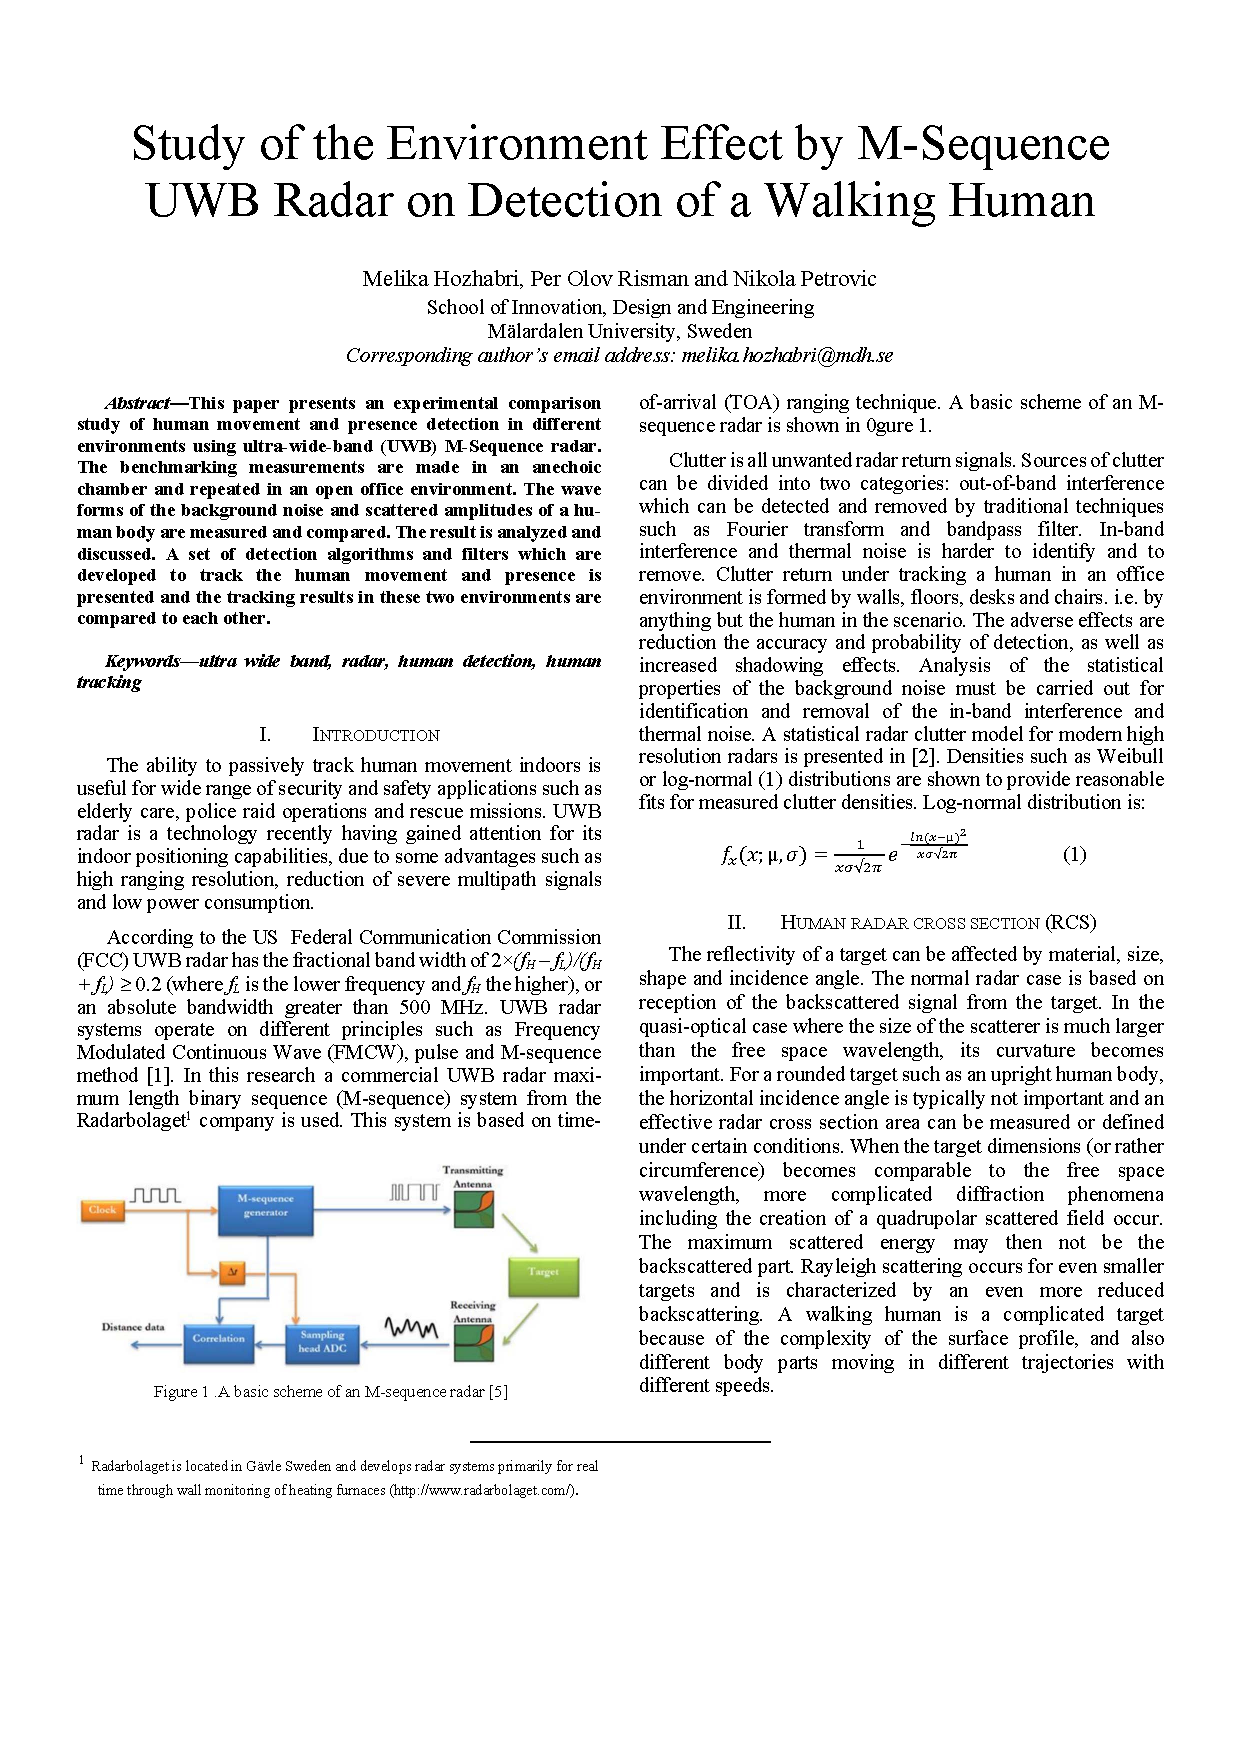
\includepdf[pages=-]{PID4411259.pdf}

\end{document}
